\pagebreak
\subsection{Thermal Design} 
\label{Thermal_section}















\subsubsection{Thermal requirements}

\paragraph{Operating temperatures}

The most obvious temperature requirement is in meeting the operating temperature for the various components, tabulated below.\\ 

% highy recommend https://www.tablesgenerator.com/

\begin{center}
\begin{table}[H]
\centering
\footnotesize
\begin{tabular}{ | l | c | c |}
    \hline
    \textbf{Component} & \textbf{Component no.} & \textbf{Operating temp [\textsuperscript{o}C]} \\ 
    \hline
    Accelerometer & KXTJ3-1057CT-ND & -40 – 85 \\ 
    \hline
    ADC AD7175 & 835-3826 & -40 – 105 \\ 
    \hline
    ADC AD7997 & 697-7170 & -40 – 85 \\ 
    \hline
    Antenna & 704-3449 & -40 – 85 \\ 
    \hline
    Buck converter 3.3V & 296-40220-1-ND & -40 – 125 \\ 
    \hline
    Buck converter 5V 4A & 785-1689-1-ND & -40 – 85 \\ 
    \hline
    Buck converter 12V 1.25A & LM2695MH/NOPB-ND & -40 – 125 \\ 
    \hline
    Camera Raspberry Pi V2 & 301-34-462 & -20 – 60 \\ 
    \hline
    Camera  ZWO ASI183MM & IMX183CLK-J & -5 – 45 \\ 
    \hline
    Capacitor 1 uF & 301-19-869 & -55 – 125 \\ 
    \hline
    Capacitor 1.4 pF & 300-47-684 & -55 – 125\\ 
    \hline
    Capacitor 22 nF & 300-65-997 & -55 – 125 \\ 
    \hline
    Capacitor 44 pF (47 pF) & 300-67-381 & -55 – 125 \\ 
    \hline
    Capacitor 850 pF & 165-81-144 & -55 – 125 \\ 
    \hline
    Capacitor 0.47 uF (420 nF) & 300-87-046 & -55 – 125 \\ 
    \hline
    Capacitor 0.1 uF & 165-73-687 & -55 – 125 \\ 
    \hline
    Capacitor 1 uF & 165-61-179 & -55 – 125 \\ 
    \hline
    Capacitor 2.2 uF & 165-71-988 & -55 – 125 \\ 
    \hline
    Capacitor 3 uF (3.3 uF) & 165-71-996 & -55 – 125 \\ 
    \hline
    Capacitor 4 uF (4.7 uF) & 300-31-816 & -55 – 125 \\ 
    \hline
    Capacitor 32 uF (33 uF) & 915-5461 & -55 – 125 \\ 
    \hline
    Capacitor 10 uF & 301-12-804 & -55 – 125 \\ 
    \hline
    Capacitor 4.7 uF & 300-31-677 & -55 – 85 \\ 
    \hline
    Capacitor 0.1 uF & 300-67-806 & -55 – 125 \\ 
    \hline
    Compass & MLX90393SLW-ABA-011 & -20 – 85 \\ 
    \hline
    Crystal 16 MHz, 9 pF, 10ppm & 301-09-485 & -40 – 85 \\
    \hline
    Encoder & 102-4485-ND & -40 – 105 \\
    \hline
    Ferrite Bead 600Ohm @ 100MHz & 724-1545 & -55 – 125 \\
    \hline
    GPS & NEO-M8N & -40 – 85\\
    \hline
    Gyroscope & EVAL-ADXRS624Z-ND & -55 – 125 \\
    \hline
    Inductor 68 uH & 300-37-257 & -40 – 105 \\
    \hline
    Inductor 24 uH (22 uH) & 158-00-313 & -20 – 105 \\
    \hline
    Inductor 22 uH & 110-63-696 & -40 – 155\\
    \hline
    Igarashi DC Gearmotor & 1711491-62 & 0 – 60 \\  
    \hline
    Microcontroller & 636-384 & -25 – 130 \\
    \hline
    Peltier cooler & PE-031-10-15-S & 0 – 74 \\
    \hline
    PWM expander & 727-5649 & -40 – 85 \\
    \hline
    Raspberry Pi Zero (no WiFi) & 1910-1104-ND & 0 – 70 \\
    \hline
    Raspberry Pi 3B+ & 137-3331 & 0 – 50 \\
    \hline
    Schottky diode & 170-09-098 & -50 – 150 \\
    \hline
    Temp sensor & 301-29-188 & -55 – 150 \\
    \hline
    Transistor NPN 15nA leak & 300-32-503 & -65 – 150 \\
    \hline
    Transistor PNP & 300-41-424 & -50 – 150 \\
    \hline
    U-regulator & 173-88-854 & -50 – 125\\
    \hline
\end{tabular}
\caption{The operating temperature for each component of the experiment.}
\end{table}
\label{tab: temp ranges}
\end{center}

As the ambient conditions are likely to be very cold, many of the components will need to be heated so that the electronics are able to operate.\\

The Igarashi DC gearmotors will need to be maintained at between 0\textsuperscript{o}C and 60\textsuperscript{o}C. If the ambient conditions are assumed to be -70\,\textsuperscript{o}C, then the temperature of these motors will need to be raised by more than 80\,\textsuperscript{o}C, assuming a tolerance of 10\,\textsuperscript{o}C.\\

The main camera (ZWO ASI183MM) will need to be maintained at between -5\textsuperscript{o}C and 45\textsuperscript{o}C. The temperature of this component will need to increase by more than 75\,\textsuperscript{o}C. Likewise for the guiding camera. For the main camera to reduce noise there is value in keeping the optics cool while the electronics are warmed to the operating temperature. This should be taken into account in the thermal design.\\

The sanity camera (Raspberry Pi Camera v2.1) will need to be maintained at between -20\textsuperscript{o}C and 60\textsuperscript{o}C. The temperature of this component will need to increase by more than 60\,\textsuperscript{o}C.\\

For the electronics box, the temperature will need to be between 0\textsuperscript{o}C and 50\textsuperscript{o}C, for the Raspberry Pi, the most temperature sensitive component. A temperature increase of more than 80\textsuperscript{o}C is required\textsuperscript{o}C.\\

\paragraph{SNR}

In order to ensure minimal measurement error in acquiring images, the effect of temperature on the optics must be considered, and the temperature must be controlled if needed to ensure that the error is within an acceptable range.\\

Dark current is small residual currents that are present in the camera, generated irrespective of whether there is incident illumination. This dark current becomes present in the data in the form of random noise that is not trivial to subtract. By decreasing the operating temperature of the camera optics, the magnitude of dark current can be minimised and the signal to noise ratio increased. This relationship between signal to noise ratio and dark current is as follows\\

\begin{center}
 $SNR =  \frac{I\times QE\times t}{\sqrt{I\times QE\times t+Nd\times t+Nr^2}}$\\
\end{center}

$I$ = Photon flux (photons/pixel/s)\\
$QE$ = Quantum efficiency\\
$t$ = Integration time (s)\\
$Nd$ = Dark current (electrons/pixel/s)\\
$Nr$ = Read noise (electrons)\\

The ASI183 camera is specified as having a read noise of 1.6e @30db gain and a QE peak of 84\%. The camera also has the following relationship between dark current and sensor temperature. Calculations will be considered for an exposure time of 300s, which is the longer intended exposure time for higher quality imaging.  \\


	\begin{figure}[h!]
    \centering
    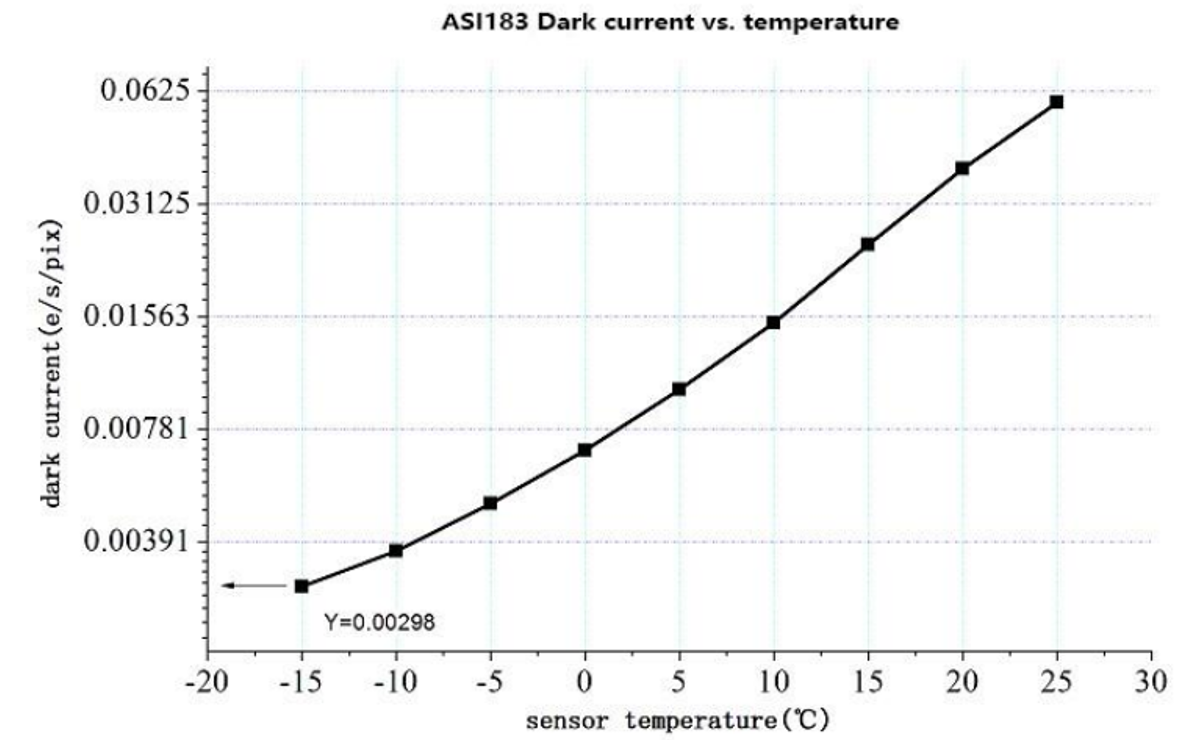
\includegraphics[scale=0.8]{4-experiment-design/img/mechanical/darkcurrent.png}
    	\caption{Dark current through the camera at various temperatures. Source: ZWO}
	\label{fig:darkcurrent}
	\end{figure}

As an example, the SNR as affected by dark current at -10\,\textsuperscript{o}C versus 10\,\textsuperscript{o}C is\\

 SNR(-10\,\textsuperscript{o}C) =  $\frac{(\SI{6.16}{photons \per pixel \per sec})\times (0.84)\times (\SI{300}{s})}{\sqrt{(\SI{6.16}{photons \per pixel \per s})\times (0.84)\times (300s)+(\SI{0.00391}{e \per pixel \per s})\times (\SI{300}{s})+(\SI{1.6}{e})^2}}$ \\

 SNR(-10\,\textsuperscript{o}C) = 39.35\\

 SNR(10\,\textsuperscript{o}C) =  $\frac{(\SI{6.16}{photons \per pixel \per sec})\times (0.84)\times (300s)}{\sqrt{(\SI{6.16}{photons \per pixel \per s})\times (0.84)\times (\SI{300}{s})+(\SI{0.01563}{e \per pixel \per s})\times (\SI{300}{s})+(\SI{1.6}{e})^2}}$ \\

 SNR(10\,\textsuperscript{o}C) = 39.31\\


\paragraph{Optothermal stability}
Another important effect will be the how thermal stresses and subsequent deflections can affect the optics of the camera, in particular the index of refraction, and hence the quality of the collected data. Variation of solar flux over the time of flight and from the heat signatures of the BEXUS module will need to be considered. A thermoelastic analysis should be conducted in finite element analysis software to evaluate the effects of the thermal environment, and the implication of those results on the validity of the data should be investigated. \

\paragraph{Condensation}
Condensation may occur if air heated by the camera heating elements is able to condensate on the cold surfaces of the optics. This will deteriorate the quality of the detections and must also be mitigated.  \

	\begin{figure}[h!]
    \centering
    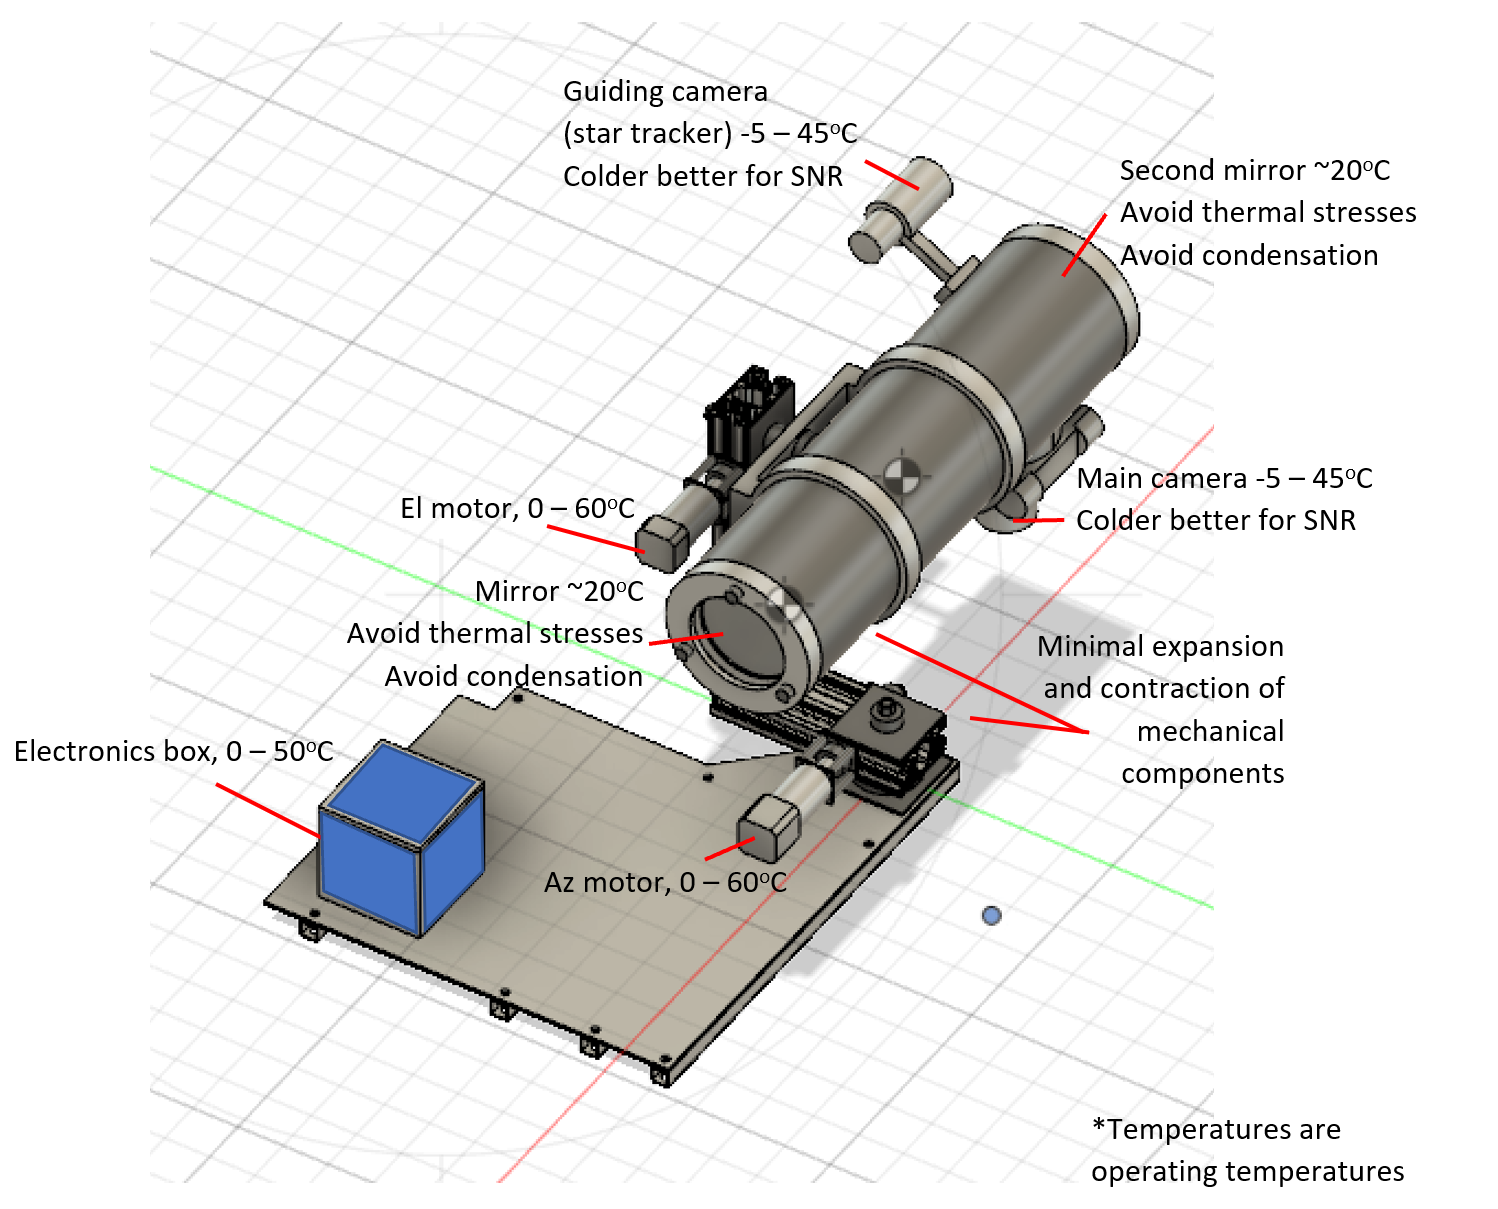
\includegraphics[scale=0.8]{4-experiment-design/img/mechanical/thermalrequirements.PNG}
    	\caption{Summary of the thermal requirements for the system.}
	\label{fig:thermalrequirements}
	\end{figure}


















\subsubsection{Thermal environment}
\paragraph{Atmosphere ambient conditions}
IRISC will ascend to and float in the stratosphere at an altitude of between 25 and 30\,km, after which it will experience altitude fluctuations of no more than 200\,m. This is the phase of flight during which the infrared camera will be operational and hence thermal control most necessary in ensuring sound optical performance. This part of the atmosphere is also characterised by relatively low temperatures. Based on the flights of number previous BEXUS missions seen in the graph of the atmosphere, it can be assumed that the atmospheric temperature during float will range between -70\,\textsuperscript{o}C and -50\,\textsuperscript{o}C. \\

	\begin{figure}[h!]
    \centering
    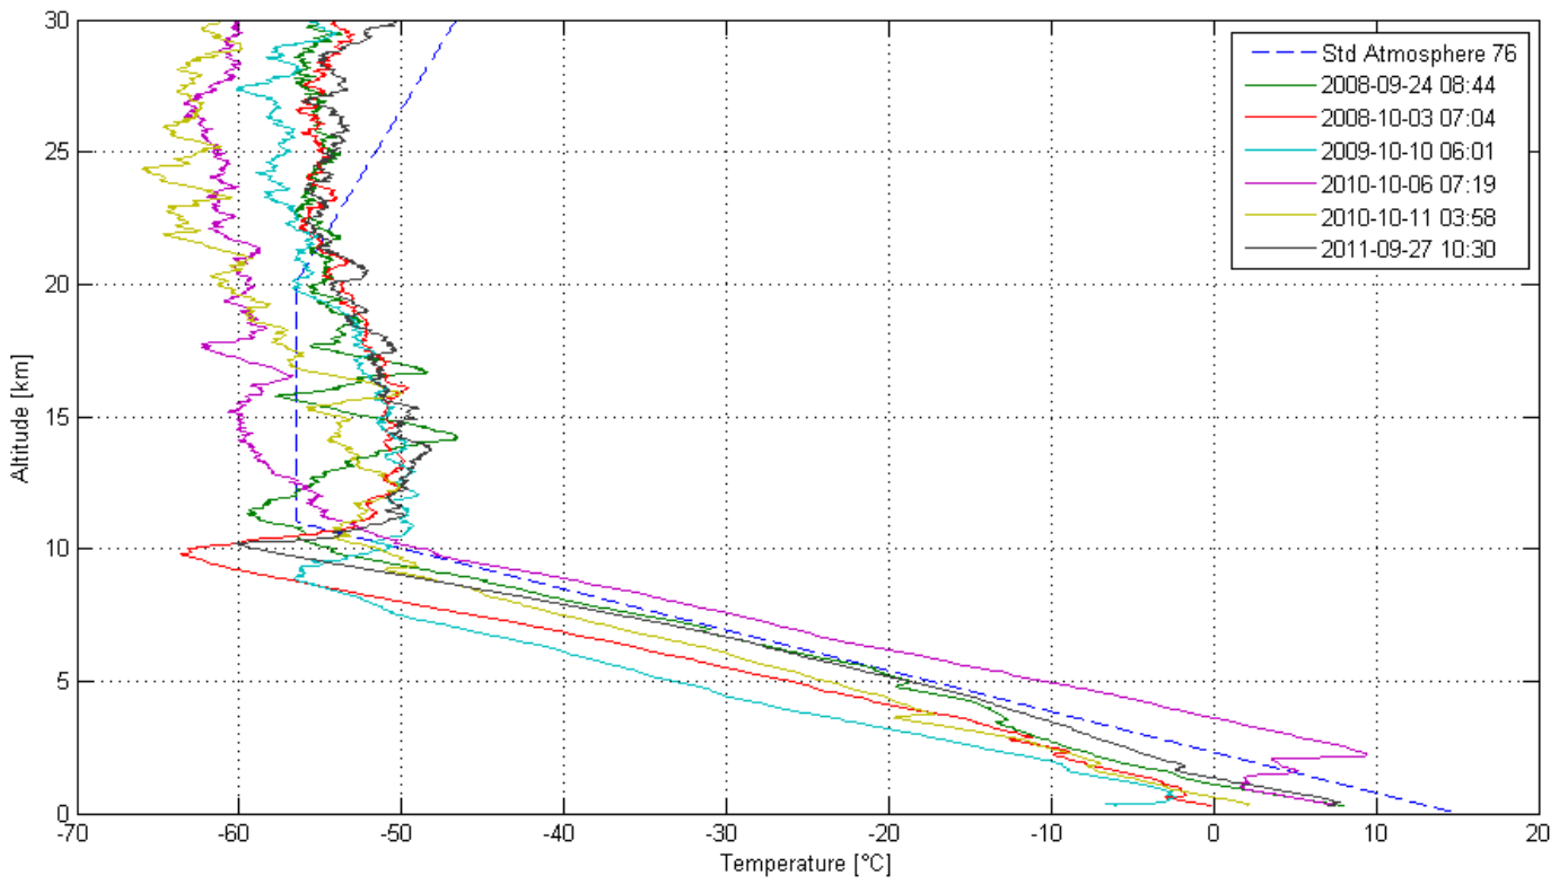
\includegraphics[scale=0.6]{4-experiment-design/img/mechanical/atmosphere.PNG}
	\caption{Temperature profile of the atmosphere. Source: REXUS/BEXUS}
	\label{fig:atmosphere}
	\end{figure}

% highy recommend https://www.tablesgenerator.com/

\begin{center}
\begin{table}
\centering
  \begin{tabular}{ | l | c | r | }
    \hline
    \textbf{Flight phase} & \textbf{Expected temperature} & \textbf{Duration} \\ \hline
    Preparation  & 15 – 25\,\textsuperscript{o}C & 4 hours \\ \hline
    Launch pad wait & -15 – 0\,\textsuperscript{o}C & 3 hours \\ \hline
    Ascent phase  & -80 – 0\,\textsuperscript{o}C & 1.5 hours \\ \hline
    Float phase (25-30km) & -70 – -50\,\textsuperscript{o}C & 1 – 5 hours \\ \hline
    Descent phase  & -80 – 0\,\textsuperscript{o}C & ~ 30 minutes \\ \hline
    Post-flight phase & -15 – 0\,\textsuperscript{o}C & 1 – 2 days \\ \hline
  \end{tabular}
\caption{\hl{The temperature expected for each phase of the BEXUS campaign.}}
\end{table}
\label{tab: flight phases}
\end{center}

\paragraph{Solar flux}

The extent of solar irradiance is characterised by several factors, including the sun’s height above the horizon, typically low for the polar latitudes that the balloon will be flying at, and the height in the atmosphere and atmospheric conditions, which will cause absorption and scattering of light. \\
The total solar irradiance, neglecting atmospheric effects, at the Esrange latitude of 68\textsuperscript{o} and assuming a launch date of the 15th of October is demonstrated in the following graph of direct solar radiation, with a peak of ~500\,W/m\textsuperscript{2} at noon.\\

	\begin{figure}[h!]
    \centering
    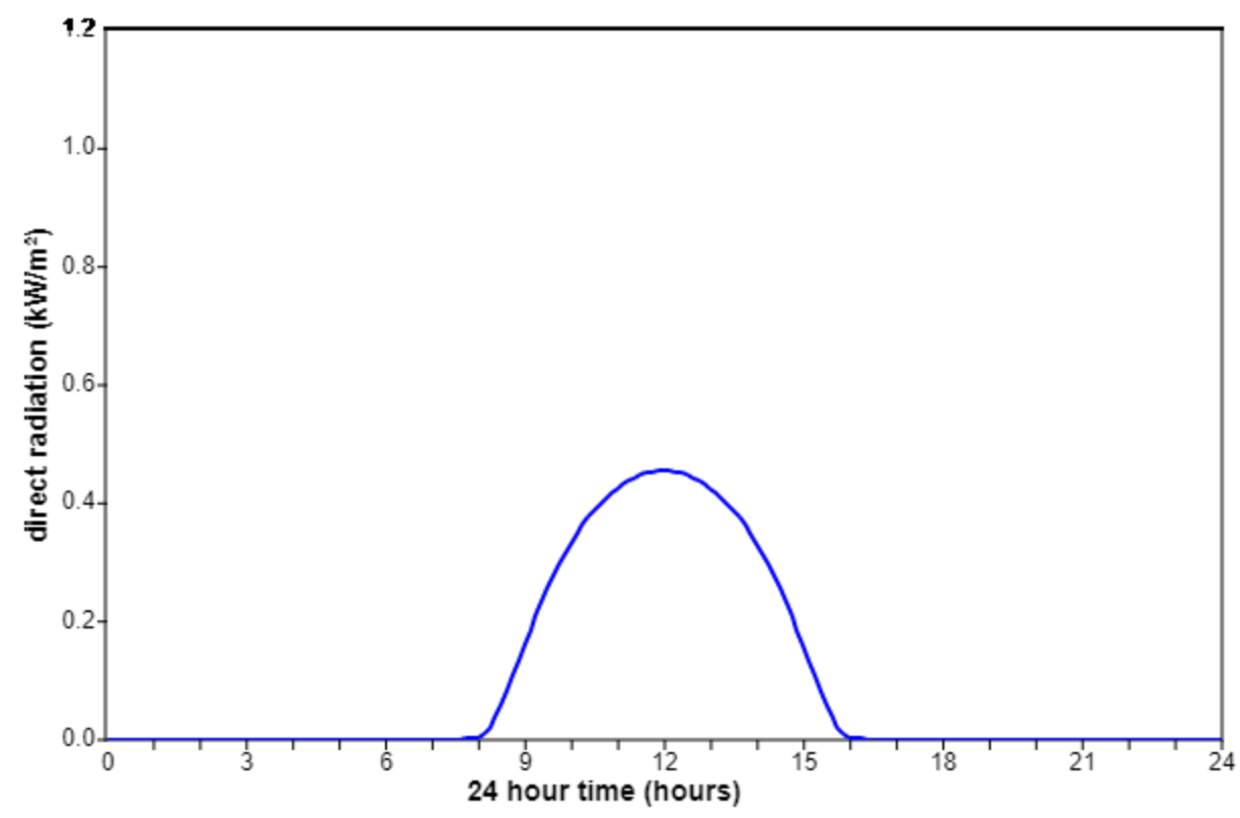
\includegraphics[scale=0.6]{4-experiment-design/img/mechanical/directradiation.png}
	\caption{Estimate of direct solar radiation at the top of the atmosphere. Source: PVeducation.org}
	\label{fig:directradiation}
	\end{figure}

The degree of attenuation of solar radiation through the atmosphere can be described using the Beer–Lambert law, which relates the transmittance of radiation to optical depth. For an atmosphere with properties that change exponentially with respect to altitude, the optical depth can be estimated to also change exponentially with respect to altitude. \\

\paragraph{Internal heat generation}
Another factor affecting the thermal environment comes from the generation of heat by the electronic components in the electronics box, from each camera, and from each motor. This heat is generated from losses of the supplied power through electrical and mechanical processes. An estimate of the power drawn by each component will be conducted.

% highy recommend https://www.tablesgenerator.com/

\begin{center}
\begin{table}
\centering
    \begin{tabular}{ | l | c | }
    \hline
    \textbf{Component} & \textbf{Power drawn [W]}\\ 
    \hline
    Raspberry Pi 3B+  & 10\\
    \hline
    Gyroscope & 0.02\\ 
    \hline
    GPS  & 0.03\\ 
    \hline
    PWM controller & 0.05\\ 
    \hline 
    Encoders  & 0.04 \\ 
    \hline
    Accelerometer  & negligible \\ 
    \hline
    Temperature sensors  & negligible \\ 
    \hline
    Buck converter 3.3V  & 0.183 \\ 
    \hline
    Buck converter 5V  & 1.67 \\ 
    \hline
    Buck converter 12V  & 3.75 \\ 
    \hline
    \textbf{Total in electronics box}  & \textbf{15.78} \\ 
    \hline
    \textbf{DC motor 1}  & \textbf{1.4} \\
    \hline
    \textbf{DC motor 2}  & \textbf{1.4} \\ 
    \hline
    \textbf{DC motor 3}  & \textbf{1.4} \\
    \hline
    \textbf{Guiding camera}  & \textbf{1.5} \\
    \hline
    \textbf{Sanity camera}  & \textbf{0.825} \\ 
    \hline
    \textbf{Main camera}  & \textbf{1.5}\\ 
    \hline
  \end{tabular}
\caption{\hl{The power drawn by each component of the experiment.}}
\end{table}
\label{tab: thermal power}
\end{center}

The DC gear motors are rated as having a maximum efficiency of 35\%. 
For electronics that consume all supplied power, such as the cameras and Raspberry Pi, all power will be converted to heat.
For other electronic components, it will be assumed that they are 90\% efficient. By multiplying the supplied power by the efficiencies, the heat generation can be determined.

% highy recommend https://www.tablesgenerator.com/

\begin{center}
\begin{table}
\centering
 \begin{tabular}{ | l | c | }
    \hline
    \textbf{Component} & \textbf{Heat generation [W]}\\ 
    \hline
    \textbf{Electronics}  & \textbf{\hl{10.58}} \\ 
    \hline
    \textbf{DC motor 1}  & \textbf{0.91} \\
    \hline
    \textbf{DC motor 2}  & \textbf{0.91} \\ 
    \hline
    \textbf{DC motor 3}  & \textbf{0.91} \\
    \hline
    \textbf{Guiding camera}  & \textbf{\hl{1.5}} \\
    \hline
    \textbf{Sanity camera}  & \textbf{\hl{0.825}} \\ 
    \hline
    \textbf{Main camera}  & \textbf{\hl{1.5}}\\ 
    \hline
  \end{tabular}
\caption{\hl{The heat generated by each component of the experiment.}}
\end{table}
\label{tab: heat generated}
\end{center}

It is of note that in historical BEXUS projects utilising the Raspberry Pi in an insulated environment, surface temperatures of 50\textsuperscript{o}C have been recorded. 





















\subsubsection{Thermal analysis}

\paragraph{Insulation}

In the electronics box, a substantial amount of heat is generated by the electrical components and in particular the Raspberry Pi. This heat will convect and radiate out to the colder surroundings. By quantifying the heat generation and comparing it to the heat losses, the temperature inside the box can be determined. The heat loss can be controlled by adding an insulating layer around the box, which will resist the conduction of energy to the surface of the box. In this case, extruded polystyrene will be used as the material, due to its low conductivity and because it is less resistant to thermal expansion. \\

An analysis of the heat loss for the electronics box maintained at 20\textsuperscript{o}C was conducted. \\

	\begin{figure}[h!]
    \centering
    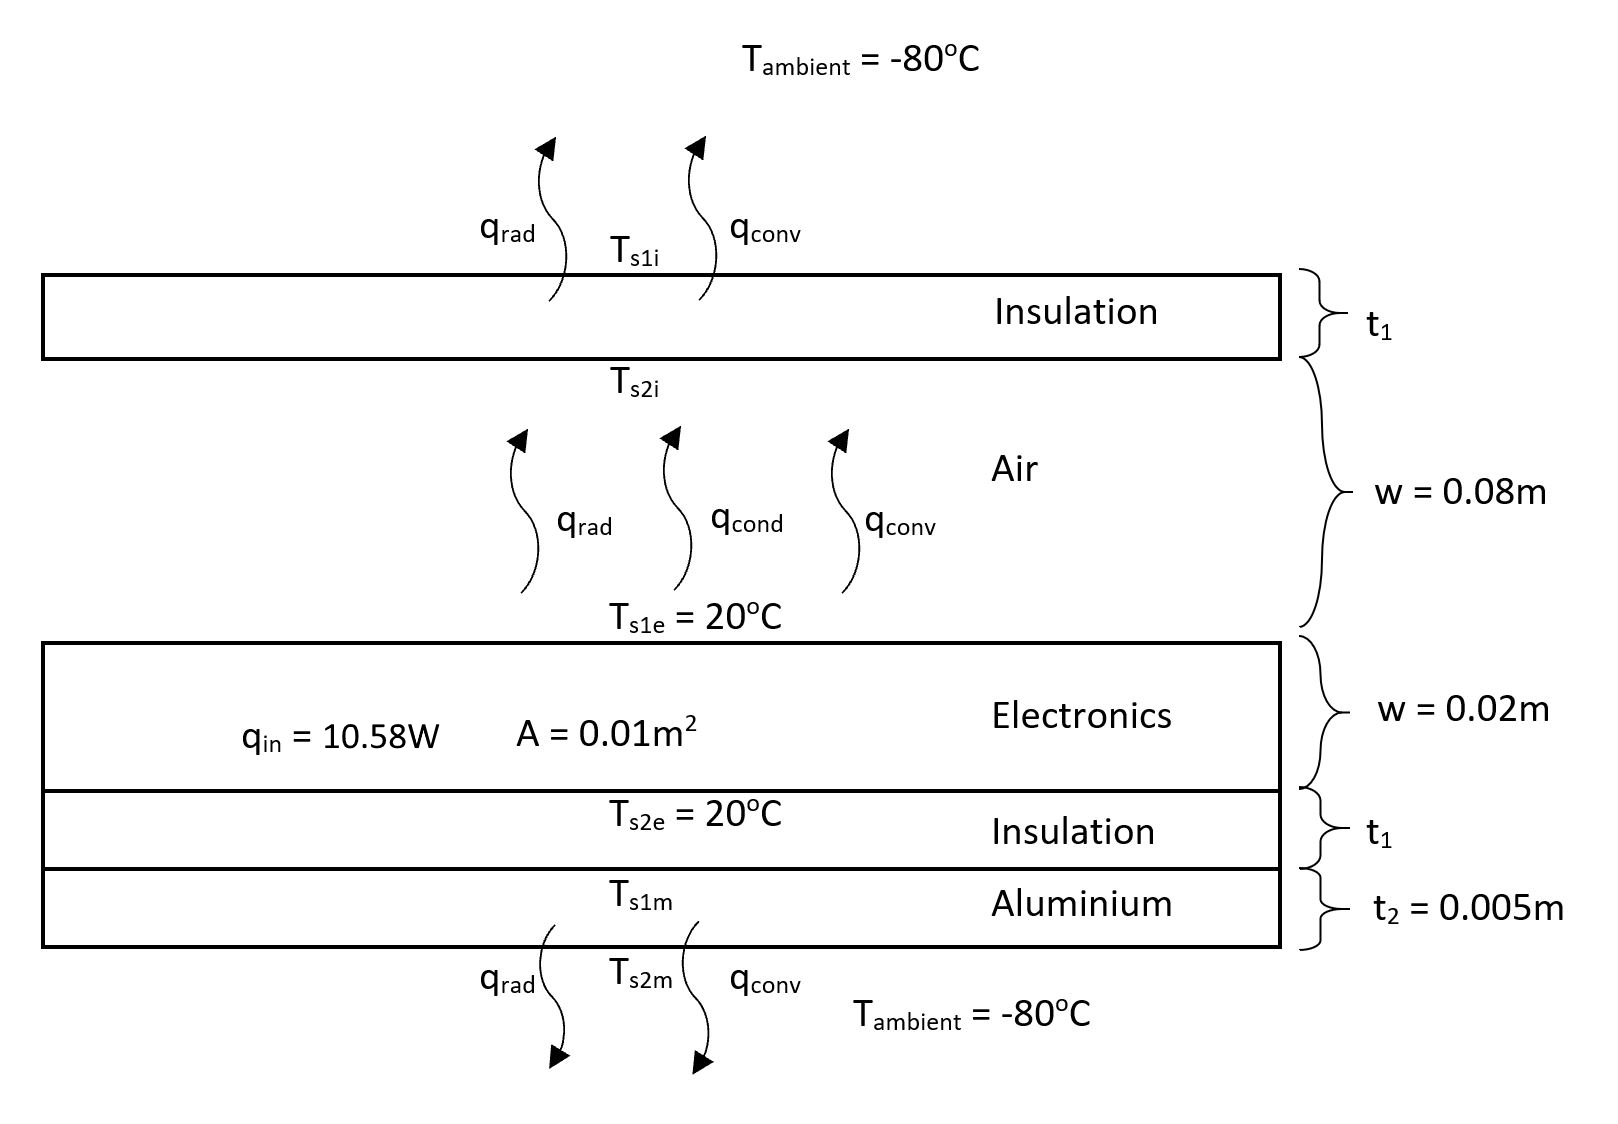
\includegraphics[scale=0.6]{4-experiment-design/img/mechanical/thermaldiagram.JPG}
	\caption{Heat transfer model of the electronics box.}
	\label{fig:thermaldiagram}
	\end{figure}

The material properties are as follows: \\

Thermal conductivity of insulation: $ k_{i} = 0.034 \frac{W}{m K} $ \\
Thermal conductivity of aluminium: $ k_{m} = 205 \frac{W}{m K} $ \\
Thermal conductivity of air at 1 kPa, -80\textsuperscript{o}C: $ k_{a} = 15\times10^{-3} \frac{W}{m K} $ \\ 
Convective heat transfer coefficient of air: $ h_{a,c} = 3.12 \frac{W}{m^{2} K} $ \\ 
Radiative heat transfer coefficient of air: $ h_{a,r} = 6.59 \frac{W}{m^{2} K} $ \\ 

For 1D steady state conduction through the composite wall comprised of insulation and aluminium: \\

	\begin{figure}[h!]
    \centering
    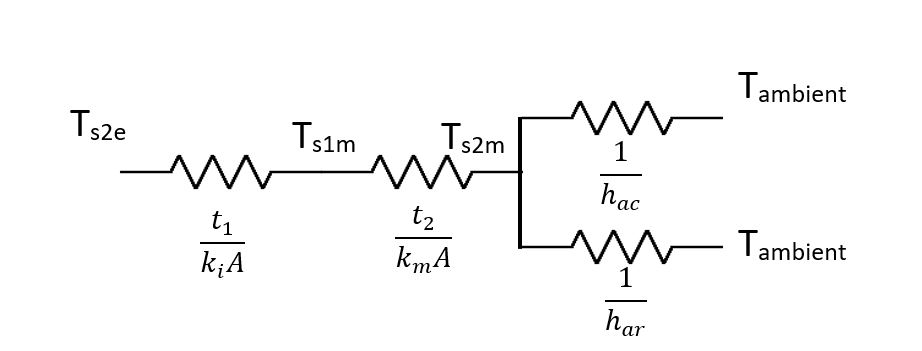
\includegraphics[scale=0.6]{4-experiment-design/img/mechanical/thermalresistance1.JPG}
	\caption{Thermal resistance for bottom of box.}
	\label{fig:thermalresistance1}
	\end{figure}

\begin{center}
 $q_{cond1} = \frac{T_{s2,e}-T_{ambient}}{R_{tot}} $\\
 
 \ 
 
 $R_{tot} = \frac{t_{1}}{k_{i}A} + \frac{t_{2}}{k_{m}A} + \frac{1}{h_{a,e}+h_{a,m}} $\\
 
 \
 \ 
 
 $q_{cond1} = \frac{293.15 - 193.15}{\frac{t_{1}}{(0.034)(0.01)} + \frac{0.005}{(205)(0.01)} + \frac{1}{3.12+6.59}} $\\
 
 \  
 \ 
 
 $q_{cond1} = \frac{100}{2940t_{1}+0.105} $\\
 
\end{center}
 

For 1D steady state conduction through the upper insulating layer: \\

	\begin{figure}[h!]
    \centering
    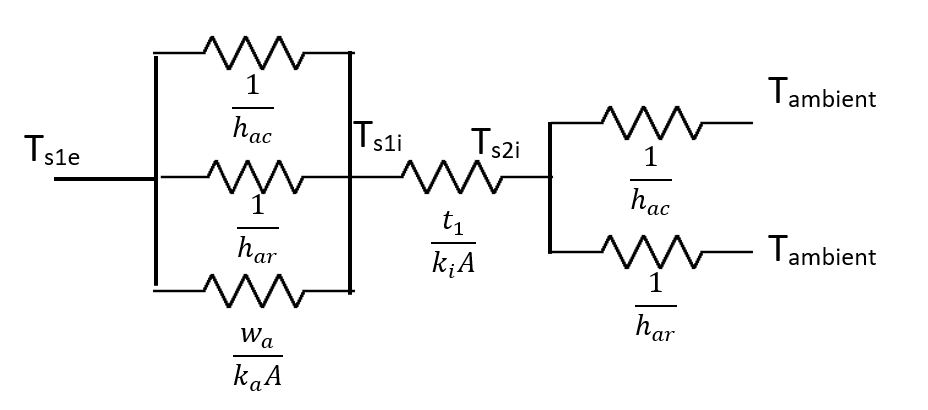
\includegraphics[scale=0.6]{4-experiment-design/img/mechanical/thermalresistance2.JPG}
	\caption{Thermal resistance for top of box.}
	\label{fig:thermalresistance2}
	\end{figure} 

\begin{center}
 $q_{cond2} = \frac{T_{s1,e}-T_{ambient}}{R_{tot}} $\\
 
 \ 
 
 $R_{tot} = \frac{1}{h_{a,e}+h_{a,m}+\frac{k_{a}A}{w_{a}}} + \frac{t_{1}}{k_{i}A} + \frac{1}{h_{a,e}+h_{a,m}}  $\\
 
 \
 \ 
 
 $q_{cond2} = \frac{293.15 - 193.15}{\frac{1}{3.12+6.59+\frac{(15\times10^{-3})(0.01)}{0.08}} + \frac{t_{1}}{(0.034)(0.01)} + \frac{1}{3.12+6.59}} $\\
 
 \  
 \ 
 
 $q_{cond2} = \frac{100}{2940t_{1}+0.206} $\\
 
\end{center}

By summing the heat lost on both sides and equating that to the heat generated, we can find the thickness of insulating material to maintain the constant temperature. \\

\begin{center}
 $q_{loss} = \frac{100}{2940t_{1}+0.105} + \frac{100}{2940t_{1}+0.206} =$ 
10.58 W
$= q_{gain} $\\
\end{center}

Solving this equation yields a thickness of 0.64\,cm. It is important to note that this analysis relies on several assumptions, such as one dimensional steady state heat transfer, and that the convection mechanism on the top and bottom of the electronics box is the same. It also does not take into account heat flux from solar radiation. In reality, there will be a conductive path through the insulating material from the bottom to the top of the box, and heat will not have to pass through the very low density air in the box. This will be taken into account in a FEA analysis of the thermal properties, using the ANSYS package. \\

To verify the results on the analytical study of the electronics box thermal scenario, a model was created and analysed using the FEA tool built into Autodesk Fusion 360. A simple model was considered, of the same dimensioned box attached to a $350 \,mm \times 450\,mm \times 6\,mm$ sheet of aluminium metal, that the box can gradually conduct heat into through the insulating material. \\

A $100\,mm \times 100\,mm \times 20\,mm$ box of epoxy resin is placed in the inside of the box, so that it is in contact with the inside walls. This box is a crude representation of the PCB, and is modelled to have the 10.58 W of heat generated uniformly through the material, representing the heat generated by the Raspberry Pi. \\

In addition to the 10.58 W of heat from the electronics box, 500 $\frac{W}{m^{2}}$ of heat was modelled as being incident on the top surface of the aluminium base and the electronics box. The system loses heat through radiation and convection of the largest surfaces to a -80\textsuperscript{o}C environment. 

The materials and corresponding properties are as follows:

% highy recommend https://www.tablesgenerator.com/

\begin{center}
\begin{table}[ht]
\centering
\resizebox{\textwidth}{!}{\begin{tabular}{ | l | c | c | c | c | c | }
    \hline
    \textbf{Material} & \textbf{Components} & \textbf{Density $ \frac{kg}{m^3} $ } & \textbf{Conductivity $ \frac{W}{m ^oC} $} &\textbf{Specific heat $ \frac{J}{^oC kg} $} & \textbf{Emissivity / absorptivity  ratio (-)} \\ \hline
    Epoxy resin  & PCB & 1140 & 0.468 & 1000 & -\\ \hline
    Aluminium & Base & 2700 & 230 & 897 & 0.46\\ \hline
    Polystyrene (extruded)  & Box, Lid & 35 & 0.027 & 1470 & 0.9\\ \hline
  \end{tabular}}
\caption{\hl{Thermal properties of the materials used in the FEA simulation, with polystyrene radiating more readily and aluminium conducting more readily.}}
\end{table}
\label{tab: thermal materials}
\end{center}

The convection constant for air, was as previously used, selected to be 3.12 $\frac{W}{m^2 K} $

A static thermal analysis was therefore conducted under these conditions, for an insulation thickness of 1 mm, 3 mm, and 6 mm. 

	\begin{figure}[h!]
    \centering	
	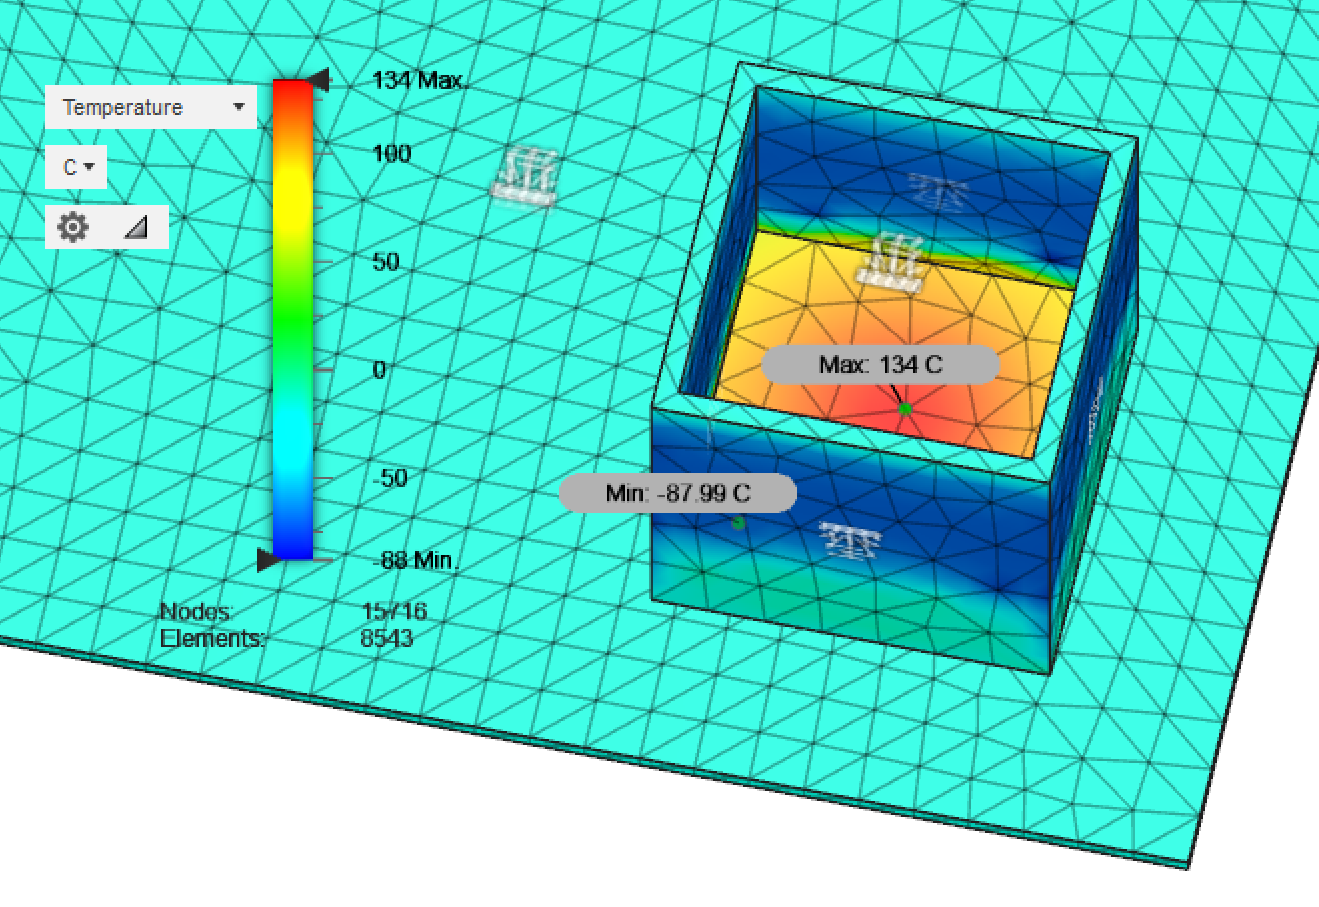
\includegraphics[scale=0.58]{4-experiment-design/img/mechanical/6mmthickheat.PNG}
	\caption{Thermal simulation of electronics box with 6mm insulation, exposed to solar heating.}
	\label{fig:6mmthickheat}
    	\end{figure}

The 6mm insulation previously recommended yields a case where temperatures are too large, 134\textsuperscript{o}C compared to the required 50\textsuperscript{o}C maximum. This makes sense, as the simplified 2D analysis did not account for the insulation material surrounding all edges of the PCB and did not account for solar heating. 

	\begin{figure}[h!]
    \centering    	
    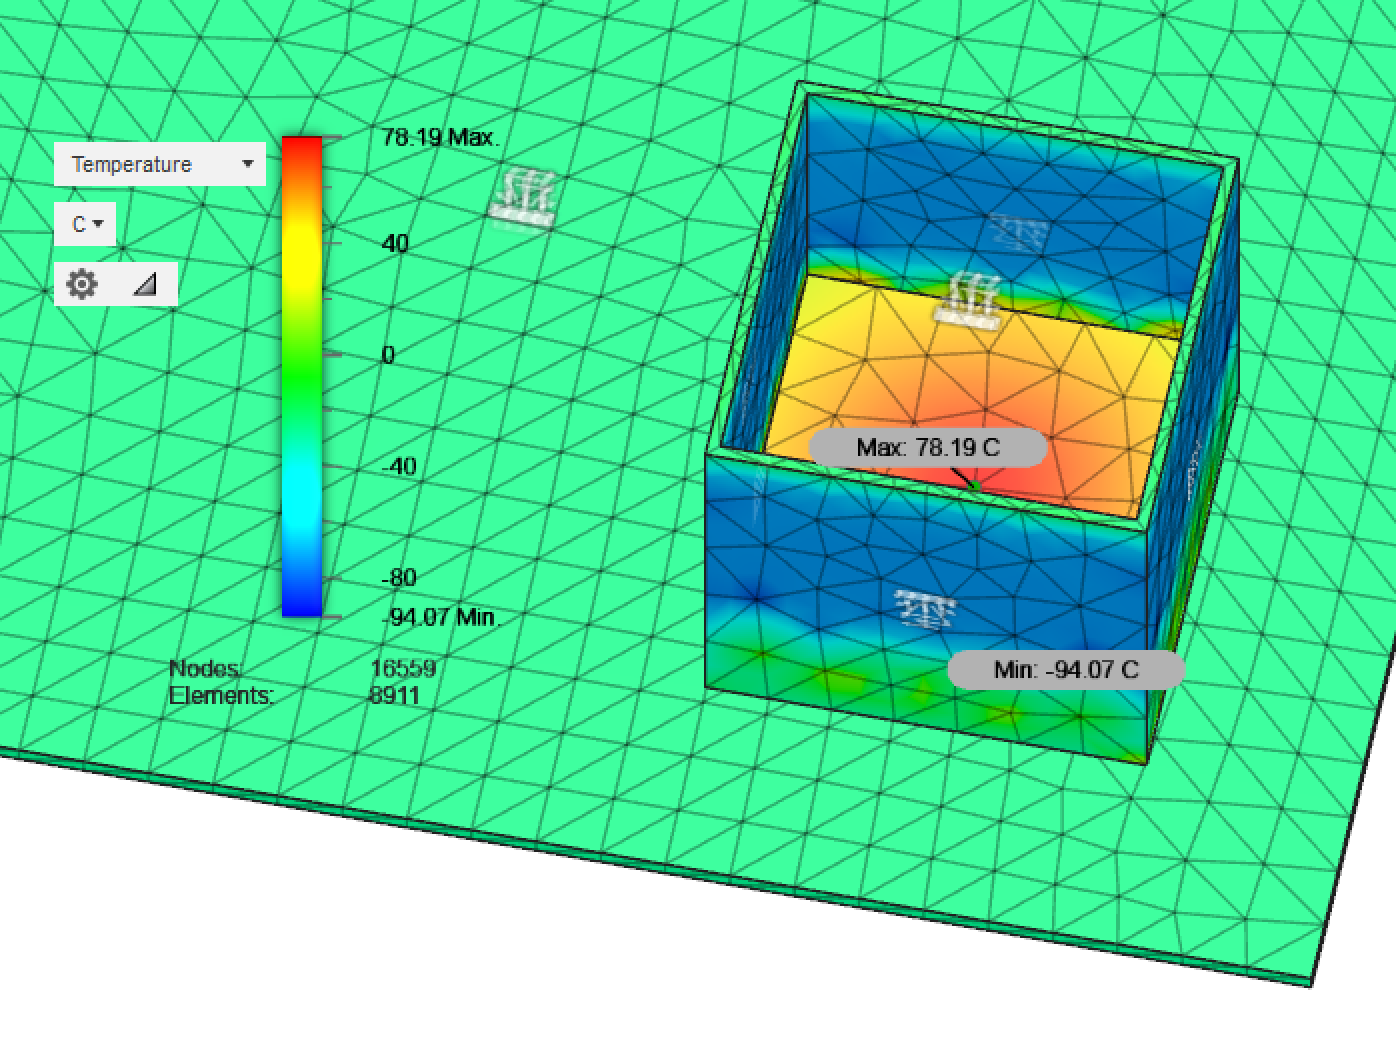
\includegraphics[scale=0.6]{4-experiment-design/img/mechanical/3mmthickheat.PNG}
	\caption{Thermal simulation of electronics box with 3mm insulation, exposed to solar heating.}
	\label{fig:3mmthickheat}
	\end{figure}

	\begin{figure}[h!]
    \centering  
    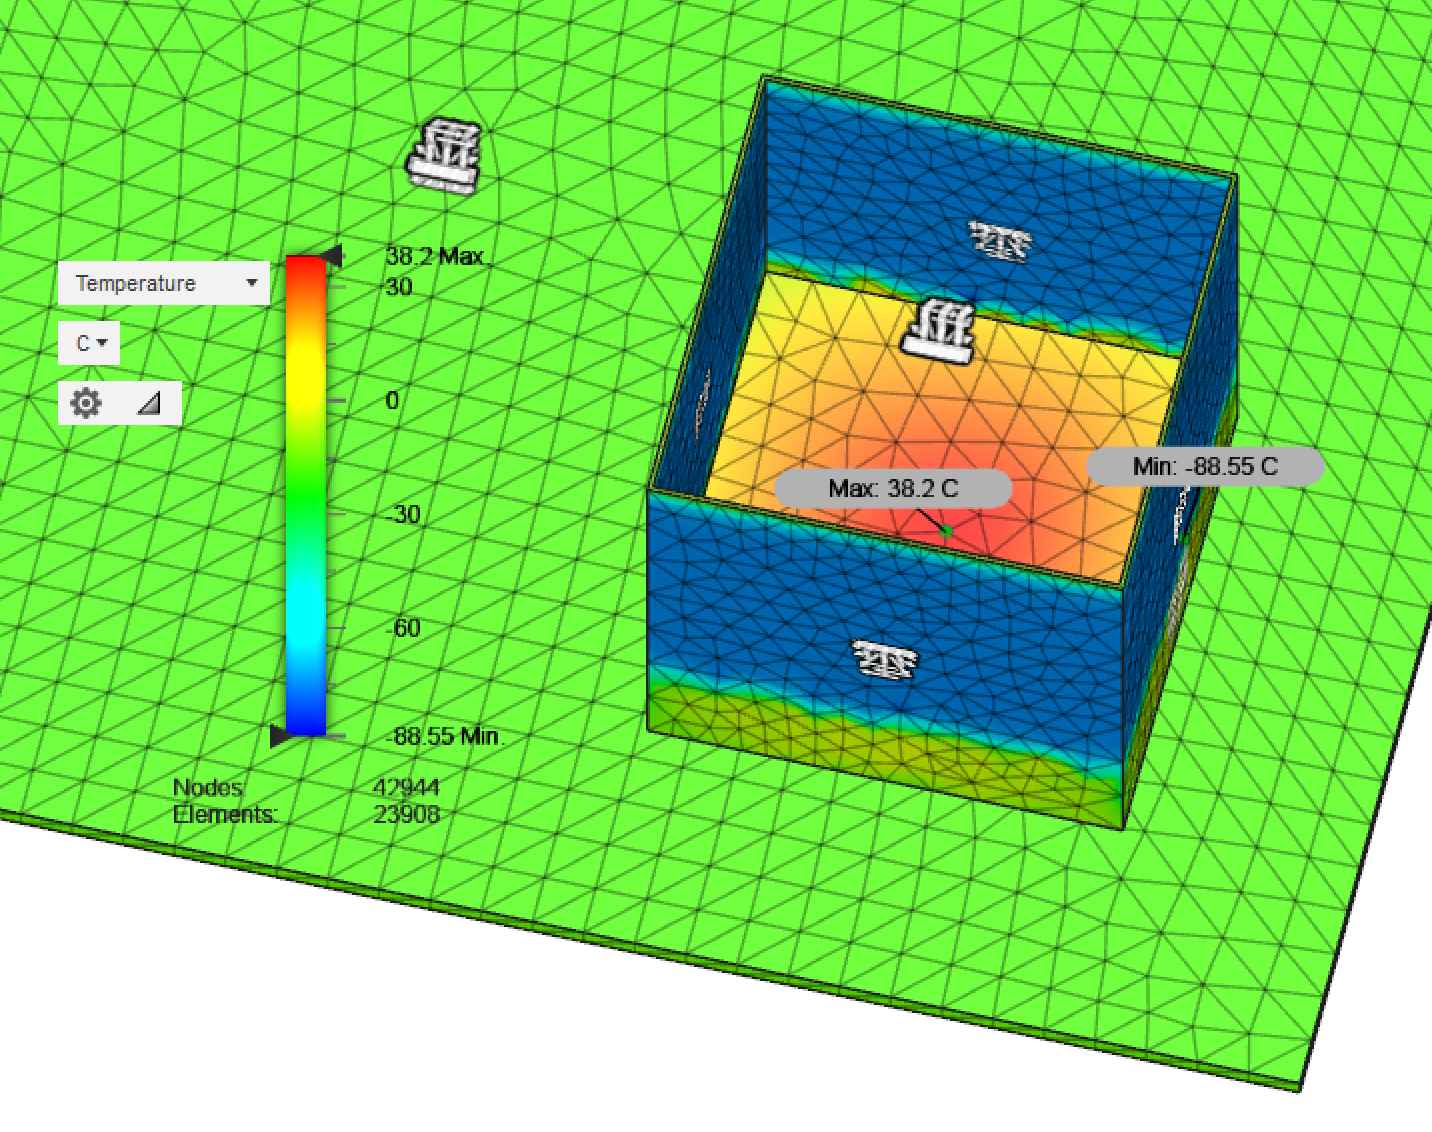
\includegraphics[scale=0.65]{4-experiment-design/img/mechanical/1mmthickheat.PNG}
	\caption{Thermal simulation of electronics box with 1mm insulation, exposed to solar heating.}
	\label{fig:1mmthickheat}    
    	\end{figure}
    	
The thermal environment was also simulated assuming no solar heating for each insulation thickness, resulting in lower temperatures. \\

	\begin{figure}[h!]
    \centering	
	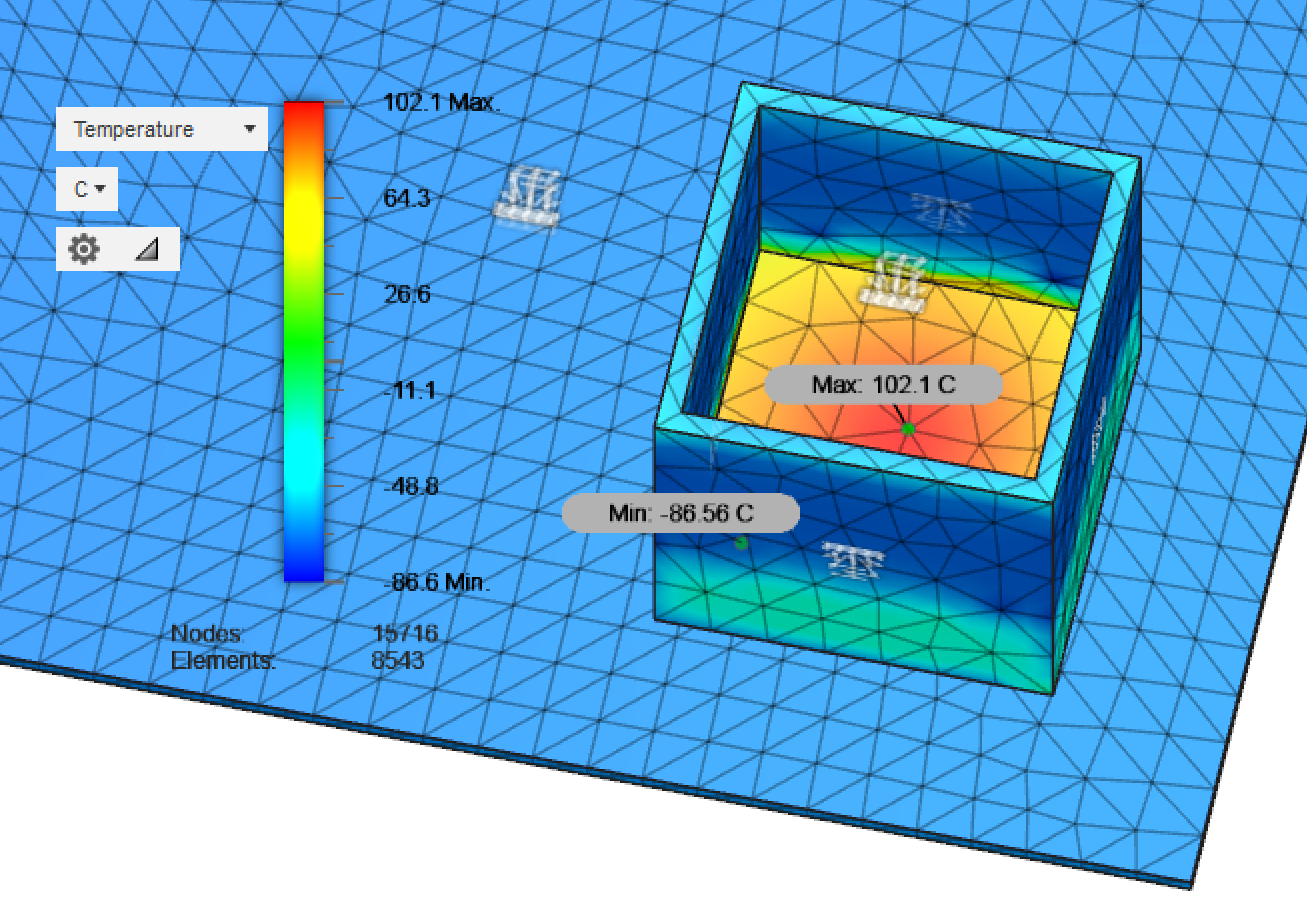
\includegraphics[scale=0.58]{4-experiment-design/img/mechanical/6mmthicknoheat.PNG}
	\caption{Thermal simulation of electronics box with 6mm insulation, no solar heating.}
	\label{fig:6mmthicknoheat}
    	\end{figure}

	\begin{figure}[h!]
    \centering    	
    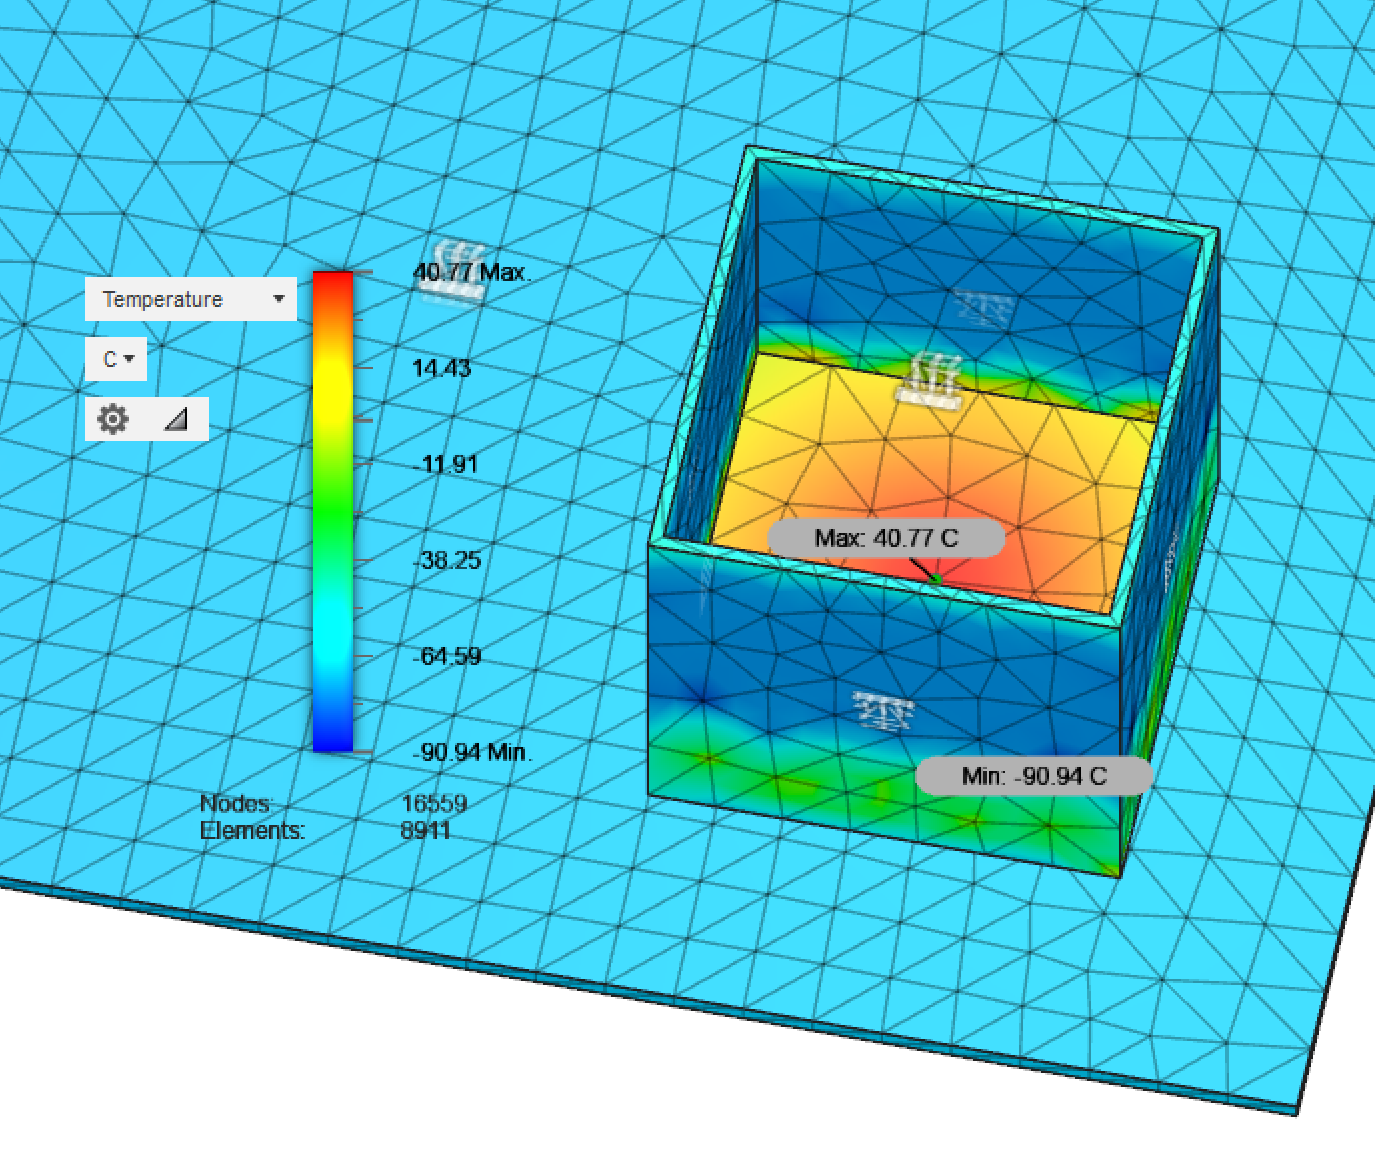
\includegraphics[scale=0.6]{4-experiment-design/img/mechanical/3mmthicknoheat.PNG}
	\caption{Thermal simulation of electronics box with 3mm insulation, no solar heating.}
	\label{fig:3mmthicknoheat}
	\end{figure}

	\begin{figure}[h!]
    \centering  
    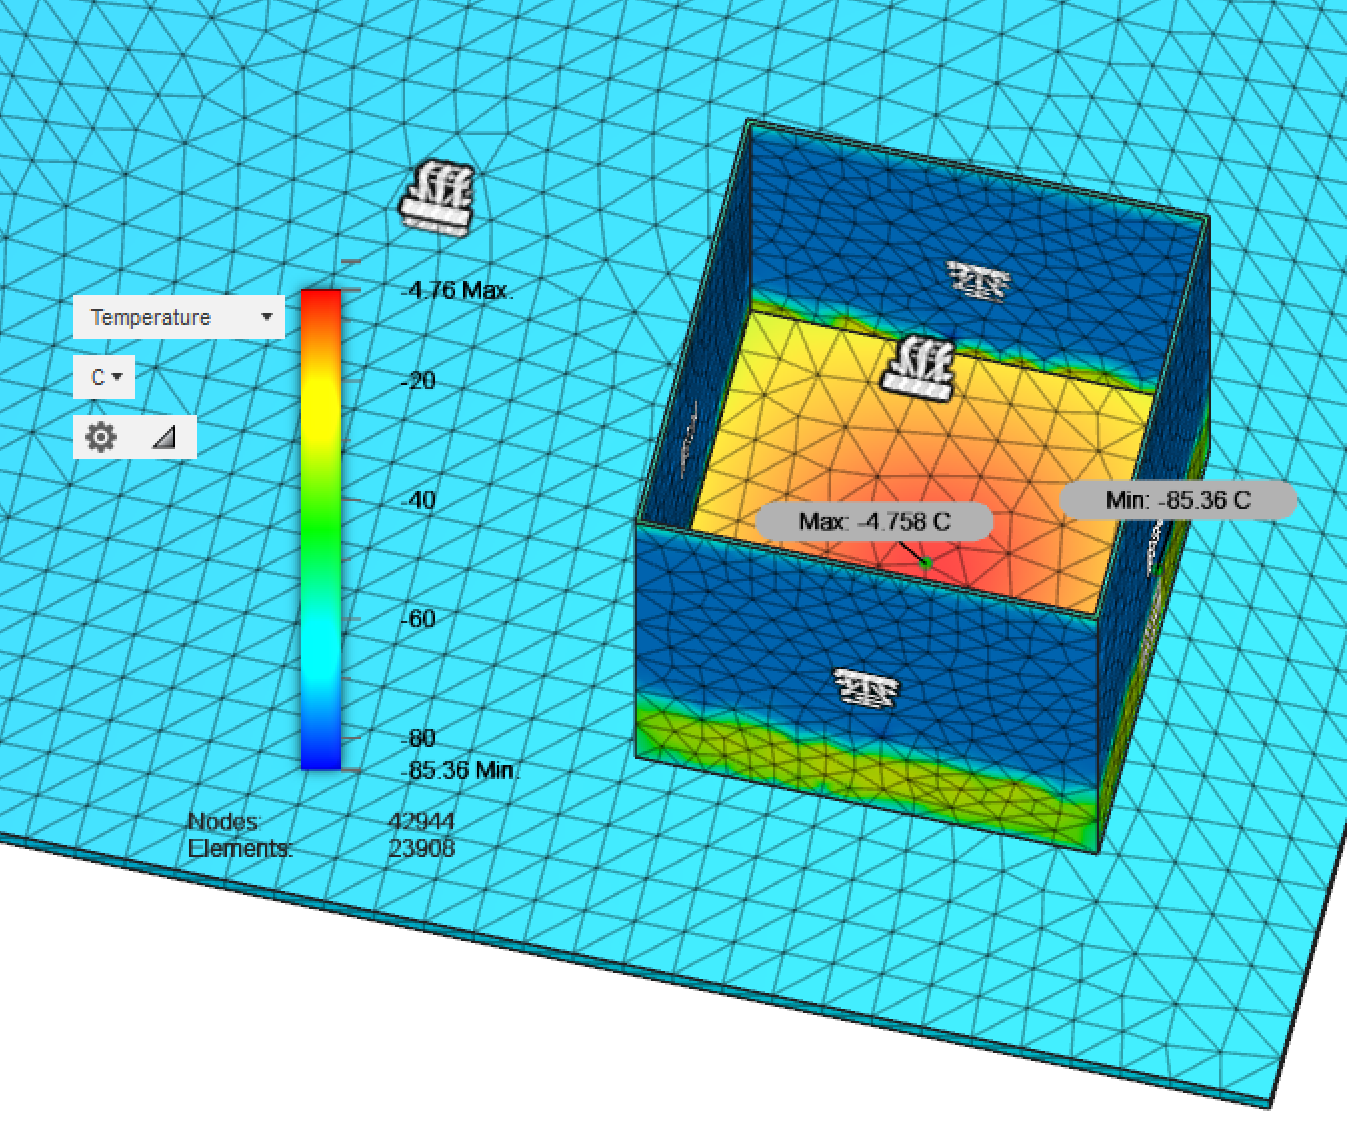
\includegraphics[scale=0.65]{4-experiment-design/img/mechanical/1mmthicknoheat.PNG}
	\caption{Thermal simulation of electronics box with 1mm insulation, no solar heating.}
	\label{fig:1mmthicknoheat}    
    	\end{figure}
	
In this case, 1mm insulation yields the best result, with the temperature at 38.2\textsuperscript{o}C with solar heating and -5\textsuperscript{o}C without, well within the required temperatures for the electronics. In any case, this analysis also makes assumptions about perfect conductive interfaces and perfect distributions of material properties, as well as a generic treatment of the thermal loads and geometry. Experimental testing will be required to ascertain more accurately the thermal conditions and to ensure that the thermal control that has been selected will work optimally and reliably. \\

Avoid electrostatic discharging 

\hl{TODOTODO}




\paragraph{Raspberry Pi heat sink}

It is also worth noting that in this analysis, the heat generated is distributed across the entire box, instead of centralised in a smaller volume, which in reality would be the case as the Raspberry Pi generates most of the heat. This would result in much higher temperatures for the Raspberry Pi, possibly exceeded ideal temperatures. Indeed, measurements taken from previous experiments have indicated temperatures at the Raspberry Pi exceeding 80\textsuperscript{o}C. \\

A small heat sink should therefore be used to distribute the heat from the Raspberry Pi more evenly, to better resemble this case. 

\paragraph{Insulation tape for telescope}
\hl{TO-DO}


\paragraph{Motors and cameras}
The motors and cameras are distinct from the electronics box in that the predicted power output is much lower, and so therefore the amount of heat able to be insulated is commensurately lower. A simple, first order estimate of the amount of insualtion needed for the motors has been conducted using a rudimentary FEA model.\\

In this model, the motors are modelled as steel cylinders generating 0.91 W of heat, surrounded by extruded polystyrene, with outer surfaces losing heat by way of radiation and convection. The same thermal environment and material properties were used as in the analysis of the electronics box.\\

	\begin{figure}[h!]
    \centering
    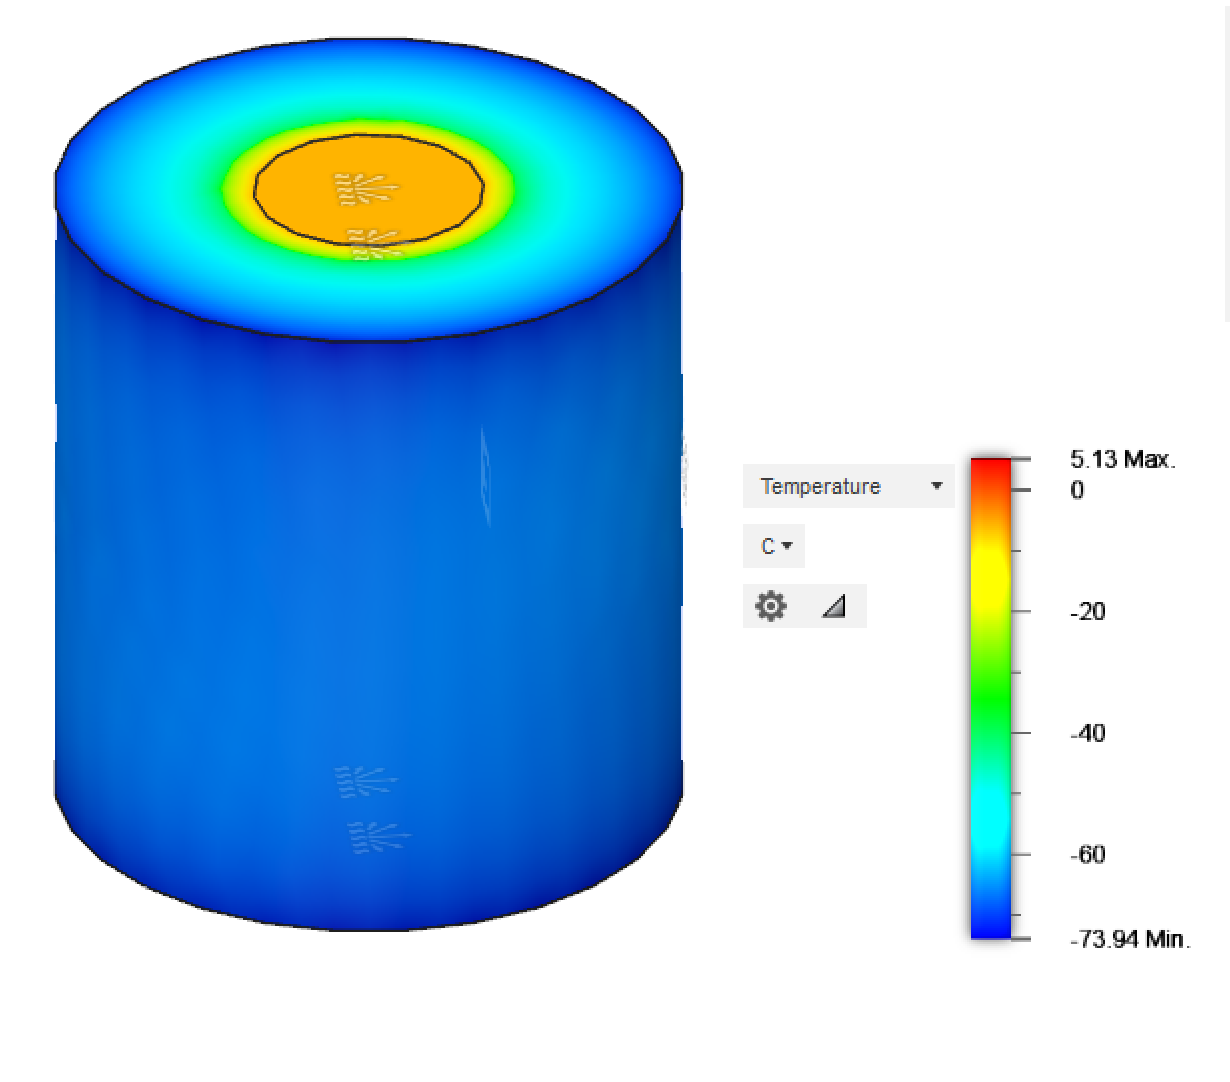
\includegraphics[scale=0.6]{4-experiment-design/img/mechanical/thermalmotors.PNG}
	\caption{Results of thermal analysis of motor with insulation and no sun shining.}
	\label{fig:thermalmotors}
	\end{figure}

It was found that in order to heat the motors to the required level, based on their heat output, a 40 mm thick layer of insulation would be needed. This seems like a large requirement, and will need to be verified with physical testing. If it is found that the amount of insulating material needs to be reduced, for spatial, mechanical, or other reasons then the heating demands can still be met by adding in heating elements to the insulated environment, which would in effect increase the total "internal heat generation" and minimise the insulation requirement.\\

For these components Minco Polyimide Thermofoil heating pads can be used. These heating pads are able to increase the temperature of a target by up to 200\textsuperscript{o}C, more than enough to reach the required temperature range for the motors and cameras given the temperatures in the stratosphere.\\

Assuming all the heat is transferred directly to the component, the power can be related to the time required to increase the target temperature by a certain amount.

\begin{center}
 $P = \frac{mC_{p}(T_{f}-T_{i})}{t} $ \\
\end{center}

For the motors with a mass of 142\,g and made of steel with a specific heat of 0.50\,J/g/$^\circ$C, to raise the temperature by 10 degrees in 5 minutes we require 2.37 W of power. It is assumed that the camera is of similar properties. \\

\begin{center}
 $P = \frac{(142)(0.5)(10\textsuperscript{o}C)}{5(60)} = \SI{2.37}{W} $ \\
\end{center}

This can be related to the resistance of the required heating pad.

\begin{center}
 $P = \frac{V\textsuperscript{2}}{R} $\\

\end{center}

By selecting the pad with resistance 52.3\,$\Omega$ and running it at 10V, it will generate 1.91W of power, and will raise the temperature by 10 degrees in 6 minutes and 11 seconds.\\ 
 
This pad is the HK5165R52.3L12, capable of supplying 15W at 28V and has dimensions 25.4\,mm x 76.2\,mm.\\

Given that the components are to be maintained at 20\textsuperscript{o}C, the maximum allowable watt density can be found, after which overheating and burning of the heating pad will occur. This will help to determine the application method of the pad to the heat sink. \\

The area of the heater is 3\,inch$^2$. Dividing the power by this area yields a power density of 0.634\,W/inch$^2$.

	\begin{figure}[h!]
    \centering
    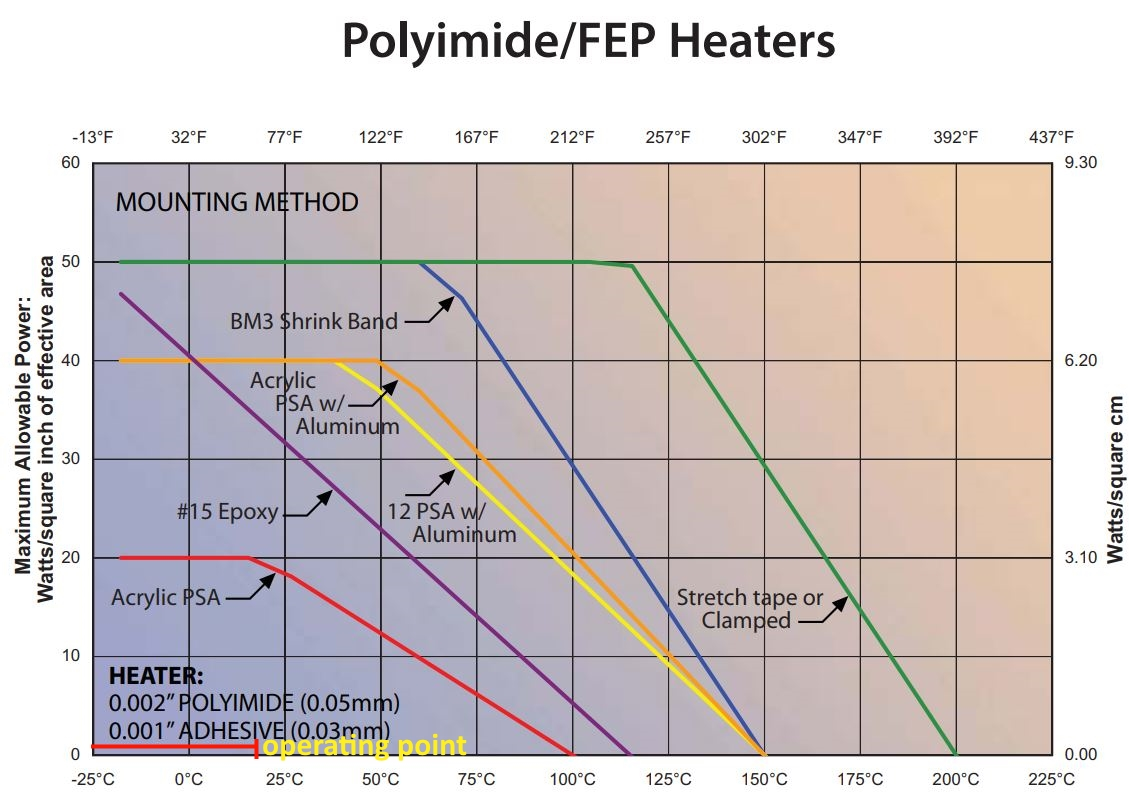
\includegraphics[scale=0.6]{4-experiment-design/img/mechanical/wattdensity.JPG}
	\caption{The maximum allowable watt density for different application methods for a given heat sink control temperature. Source: Minco heaters}
	\label{fig:thermalresistance1}
	\end{figure}

As this is low that burning of the heater is unlikely to occur, unless the temperature is not properly regulated and the heating pad warms well beyond the desired control temperature. Also, any application method is suitable with respect to this concern. To ensure proper conduction onto the surfaces of the motors and cameras, a thermal interface pad (ILA-TIM-CLUSTER-30X30-2A) will be used ensuring no air gaps that can cause spot heating or electric sparking. \\


\subsubsection{Thermal control}
The following methods for regulating the thermal environment have been suggested:\\

\begin{itemize}
  \item Extruded polystyrene to insulate electronics box self-heat. 
  \item Heat sink for the Raspberry Pi in the electronics box.
  \item White reflecting tape, few conductive pathways for the telescope optics.
  \item Insulation tape, small conductive pathways to isolate telescope optics.
  \item Extruded polystyrene and Minco heaters to heat motors and cameras.

\end{itemize}

\begin{figure}[h!]
\centering
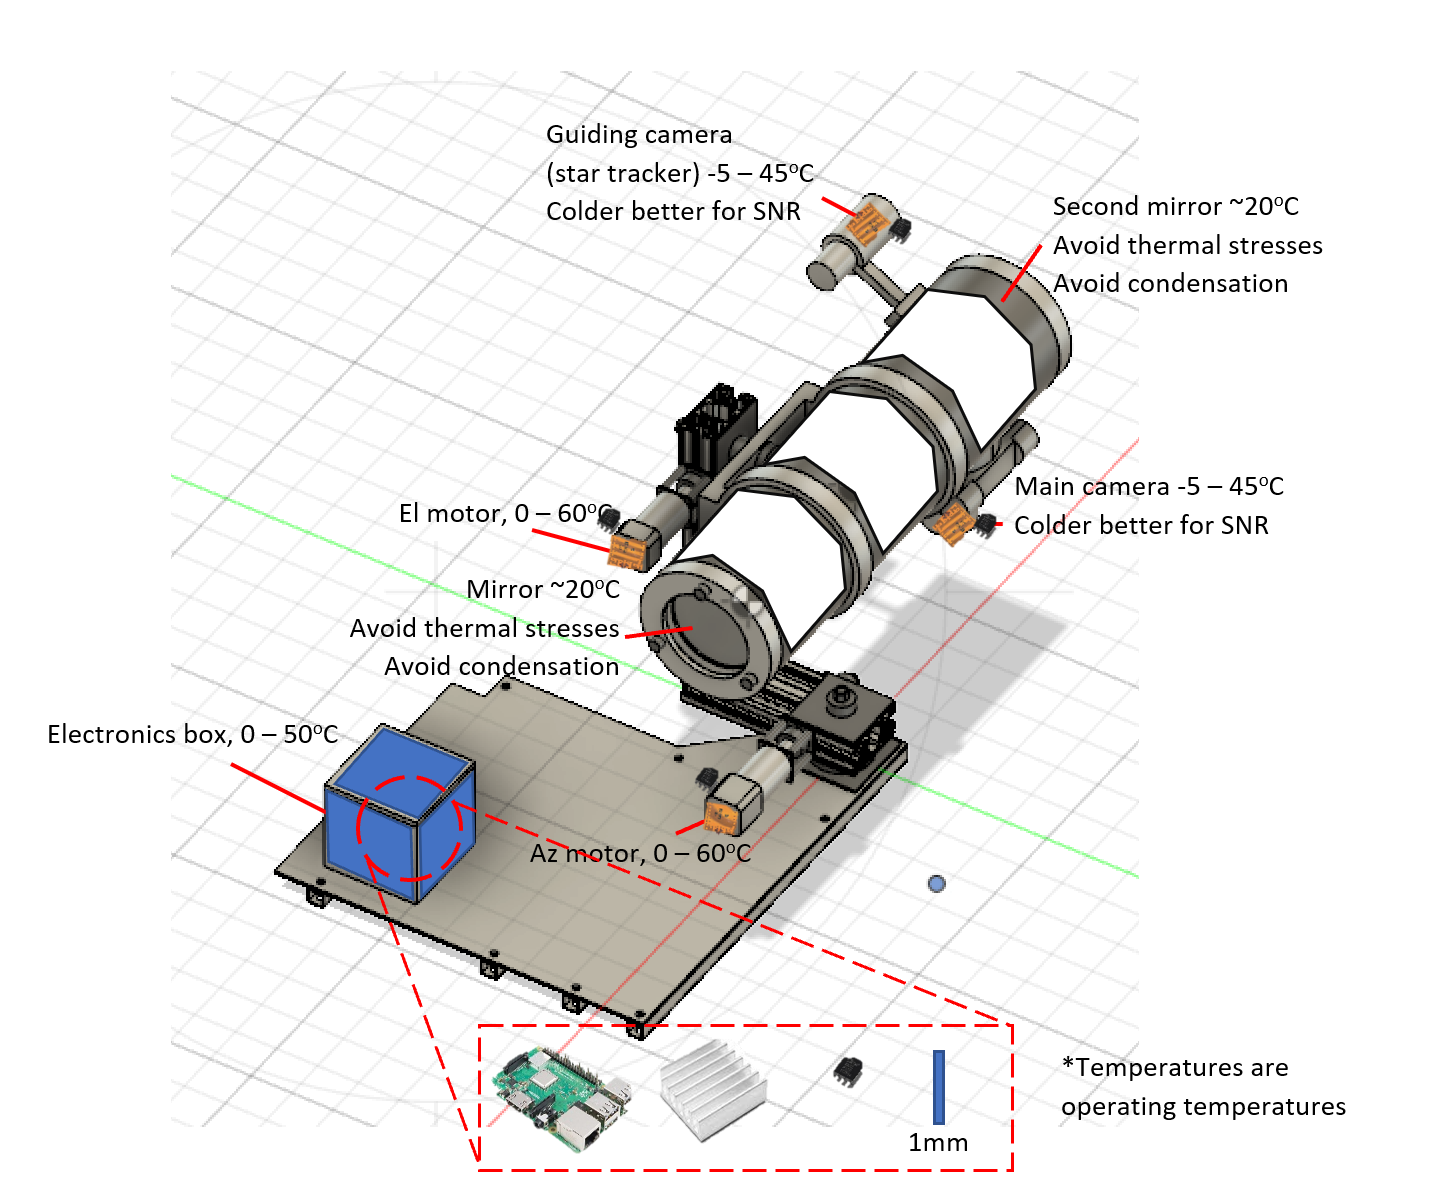
\includegraphics[scale=0.8]{4-experiment-design/img/mechanical/thermalsolutions.png}
\caption{Summary of the thermal control mechanisms for the system.}
\label{fig:thermalsolutions}
\end{figure}

Risks have been identified and addressed including:

\begin{itemize}
  \item Electrostatic charging from movement of the polystyrene or PCBs.
  \item Overheating of the Raspberry Pi. 
  \item Deformation of the mirrors. 
  \item Air gaps between heaters and motors leading to spot heating. 
  \item Air gaps between heaters and motors leading to electrical sparking.

\end{itemize}

To measure the temperature of the motors and especially cameras, which should be kept on the cooler end of the operating range, four Adafruit 165 temperature sensors will be used. This output will be fed into a simple proportional control loop to keep the components within the desired temperature range. Precision is not a major requirement for the thermal system. 

